\subsection{Artificial Neural Networks}
\textit{Artificial neural networks} (\textit{ANNs}), sometimes referred to as \textit{neural networks} (\textit{NNs}), are a category of bio-inspired algorithms that are structured like and can learn similarly to a brain. They are the foundation to many modern machine learning systems. Early concepts have been developed in 1943 \cite{first-neuron}, but they were not widely applicable due to the lack of computational resources. However, today, even consumer grade graphics cards intended for video games are powerful enough to run complex neural network models and are starting to be engineered specifically to accelerate machine learning applications \cite{tensor-cores}.

At their core, artificial neural networks are function approximators. Say, for example, we want to predict the output of a function $g$ without knowledge of its inner workings. Instead, we are only given several input-output samples produced by $g$. In this case, we may use a neural network, which, given a set of parameters $\theta$, also produces an input-output mapping $f_\theta$ that likely is not similar to $g$ by default. We now iteratively adjust $\theta$ using the input-output samples created by $g$ so that $f_\theta$ also produces (close to) the same outputs. The network is then expected to behave similarly to $g$ for previously unknown inputs.

The fundamental unit of neural network is often the McCulloch-Pitts neuron \cite{first-neuron}. Inspired by biological neurons, McCulloch-Pitts mathematical neurons receive a vector of real-valued inputs $x = (x_1, ..., x_n)$, which are weighted with parameters $w = (w_1, ..., w_n)$ and then summed to produce a single real-valued output. This output is then further transformed by an \textit{activation function} $h$, allowing the neuron to produce non-linear mappings. A \textit{threshold} term or \textit{bias} $b$ is usually introduced as well, creating the equation:
\begin{equation*}
    y = h\left(\sum_{i=1}^n w_i x_i + b \right)
\end{equation*}
Possible activation functions include \textit{sigmoid}, \textit{tanh} or \textit{ReLU}\footnote{Rectified Linear Unit}. The full neuron can be seen in figure \ref{fig:neuron}.
\begin{figure}[ht]
    \centering
    \begin{subfigure}{0.49\textwidth}
        \raggedright
        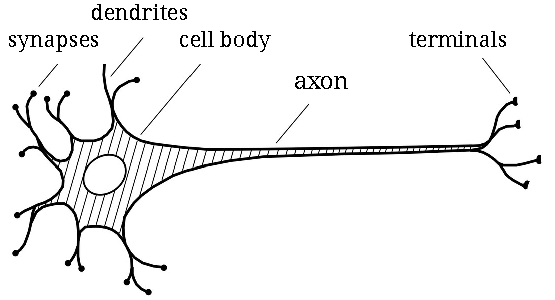
\includegraphics[width=\textwidth]{assets/bio_neuron.pdf}
    \end{subfigure}
    \begin{subfigure}{0.5\textwidth}
        \raggedleft
        \begin{tikzpicture}
            \node (x1) {$x_1$};
            \node [below = 0.25 of x1] (x2) {$x_2$};
            \node [below = 0.25 of x2] (x3) {$x_3$};
            \node [below = 0.15 of x3] (xdot) {\vdots};
            \node [below = 0.35 of xdot] (xn) {$x_n$};

            \node [right = of x3, draw, circle] (sum) {$\sum$};

            \node [above = of sum] (bias) {$b$};

            \node [right = 0.5 of sum, draw, rectangle] (activation) {$h$};
            \node [right = of activation] (y) {$y$};

            \draw [->] (x1) -- (sum);
            \draw [->] (x2) -- (sum);
            \draw [->] (x3) -- (sum);
            \draw [->] (xn) -- (sum);

            \draw [->] (bias) -- (sum);

            \draw [->] (sum) -- (activation);
            \draw [->] (activation) -- (y);
        \end{tikzpicture}
    \end{subfigure}
    \caption{Comparisson of a biological neuron \cite{bio-neuron} (left) and a mathematical McCulloch-Pitts neuron (right).}
    \label{fig:neuron}
\end{figure}
Individual units were later put together to form the \textit{perceptron} \cite{first-perceptron}. Multiple layers of neurons are called \textit{multi-layer perceptron}. Having many of such layers popularized the terms \textit{deep neural network} and \textit{deep learning}.

Perceptrons can be trained using gradient descent of an error (or \textit{loss}) term with respect to its parameters $\theta$, which is referred to as \textit{back-propagation} \cite{back-propagation}. Calculating gradients for each neuron in a complex model is difficult and is required to be highly optimized. Programming libraries such as \textit{TensorFlow} \cite{tensorflow} or \textit{PyTorch} \cite{pytorch} solve this issue by performing automatic differentiation and parallelizing mathematical operations on the GPU.

\subsubsection{Deep Reinforcement Learning}
The advancements in artificial neural networks and deep learning have also spawned a new era of reinforcement learning algorithms that use neural networks as function approximators.

The first published \textit{Deep Reinforcement Learning} algorithm was \textit{Deep Q-learning} (\textit{DQN}) \cite{dqn}, a variation of the Q-learning algorithm that uses an artificial neural network called \textit{Q-network} instead of a Q-table. It also introduced \textit{Experience Replay}, a system in which past experience of an agent is stored in a \textit{replay buffer} so as to make the training process more robust. DQN achieved state-of-the-art, super-human performance in several video games from the \textit{Atari 2600 console}, receiving only the very high dimensional visual information from the game screen as observations.

Over the years, several improvements have been made to the original DQN. For instance, \textit{Double DQN} \cite{double-dqn} uses two neural networks to mitigate DQN's tendency to overestimate action-values. \textit{Prioritized Experience Replay} (\textit{PER}) \cite{per} weighs experience samples from the replay buffer differently based on how good the model already is at correctly estimating their values. For example, an experience sample that is hard for the neural network to learn is chosen more often for training. The \textit{Rainbow} algorithm \cite{rainbow} combines a variety of individual improvements to DQN and manages to significantly outperform each individual improvement.

Actor-critic architectures have also been enhanced with deep neural networks. Notably, the \textit{asynchronous advantage actor-critic} (\textit{A3C}) \cite{a3c} achieved state-of-the-art results even when compared to DQN and can handle continuous state and action spaces. It works by letting several copies of the agent interact with seperate environment instances asynchronously, and combining the gathered experience for training. Similarly to DQN, A3C has received several modifications over the years. For example, the \textit{actor-critic with experience replay} (\textit{ACER}) \cite{acer} improves the sample efficiency of A3C by introducing Experience Replay to the otherwise on-policy algorithm.